%% LyX 2.0.3 created this file.  For more info, see http://www.lyx.org/.
%% Do not edit unless you really know what you are doing.
\documentclass[english]{article}
\usepackage{mathptmx}
\usepackage{helvet}
\usepackage{courier}
\usepackage[T1]{fontenc}
\usepackage[latin9]{inputenc}
\usepackage{listings}
\usepackage{geometry}
\geometry{verbose,tmargin=2.54cm,bmargin=2.54cm,lmargin=2.54cm,rmargin=2.54cm}
\usepackage{float}
\usepackage{graphicx}

\makeatletter

%%%%%%%%%%%%%%%%%%%%%%%%%%%%%% LyX specific LaTeX commands.
\floatstyle{ruled}
\newfloat{algorithm}{tbp}{loa}
\providecommand{\algorithmname}{Algorithm}
\floatname{algorithm}{\protect\algorithmname}

\makeatother

\usepackage{babel}
\begin{document}

\title{Finding conserved transcription factor binding sites by comparing
ChIP-seq experiments}


\author{Colin Diesh}


\date{Senior Thesis Project, Fall 2012\\
$\,$\\
First semester final report}
\maketitle
\begin{abstract}
DNA-protein interactions are essential for gene regulation, and these
interactions can be detected by using chromatin immunoprecipitation
and high throughput sequencing (ChIP-seq). Transcription factors in
particular are proteins that bind to specific sequences on the DNA,
thereby promoting or suppressing the transcription of nearby genes.
Using ChIP-seq, transcription factor binding sites are identified
as peaks in the data that represents a \textquoteleft{}tag pileup\textquoteright{}
of DNA sequences. Some binding sites have too weak of a signal to
confidently identify, but evidence from comparing ChIP-seq experiments
from the genomes of related strains may provide the additional support
needed to identify these. We found substantial evidence for weak binding
sites that are conserved but aren\textquoteright{}t found by other
peak finding algorithms, and we use a normalized difference score
described by Zheng et al (2010) to find some of these. We also introduce
a modified normalized difference score that uses data from multiple
genomes concurrently.
\end{abstract}

\section{Introduction}

The genes in our DNA are regulated by a variety of proteins that interact
and bind with the DNA. Transcription factors in particular are proteins
that can affect DNA transcription by binding to the DNA, thereby regulating
nearby genes. Transcription factors bind to a particular DNA motif,
which is a short DNA sequence that they are attracted to. Identifying
the transcription factor binding sites has become an important problem
for understanding gene regulation. However, comparisons of different
related species have shown a high degree of variability of binding
sites in human and mouse and in different strains of yeast (Odom et
al. 2003, Zheng et al. 2010). 

ChIP-seq is a next-generation sequencing method for detecting DNA-protein
interactions. ChIP-seq uses chromatin immunoprecipitation followed
by high throughput sequencing to find DNA sequences to which transcription
factors bind. ChIP-seq data is made up of many short DNA sequences,
and after the sequences are aligned to a reference genome, the transcription
factor binding sites appear as \textquoteleft{}peaks\textquoteright{}
in the data. Peak finding algorithms use a significance level that
is based on a somewhat arbitrary threshold. 

In order to compare ChIP-seq data, typically, the binding sites from
different experiments are identified from each experiment individually,
and if the location of a binding sites overlap at the same genome
position in each experiment, then they are shared. If the comparison
involves comparing different genomes, then we can either compare nearby
genes of the binding sites if there exist homologous genes to compare.
Other techniques for comparing binding sites from different genomes
use a DNA alignment of each genome to find overlapping binding sites.
Odom et al. (2007) developed a peak classification that uses DNA alignment
and the ChIP signal to compare human and mouse binding sites which
illustrates how binding sites can vary from comparing different genomes.

Using the peak classification, conserved binding sites are defined
as binding sites that have the same target gene which also have conserved
DNA alignments. The conserved DNA alignment is typically characterized
using motif finding (Odom et al. 2007) but they can also use multiple
sequence alignments (Moses et al. 2004). A gained or lost peak will
have conserved sequences, but they will not have similar peak characteristics.
The unaligned and turnover classes of peaks will not have a matching
the sequence alignment, \textquotedblleft{}so they can not be classified
definitely\textquotedblright{} (Odom et al. 2007).

\begin{figure}


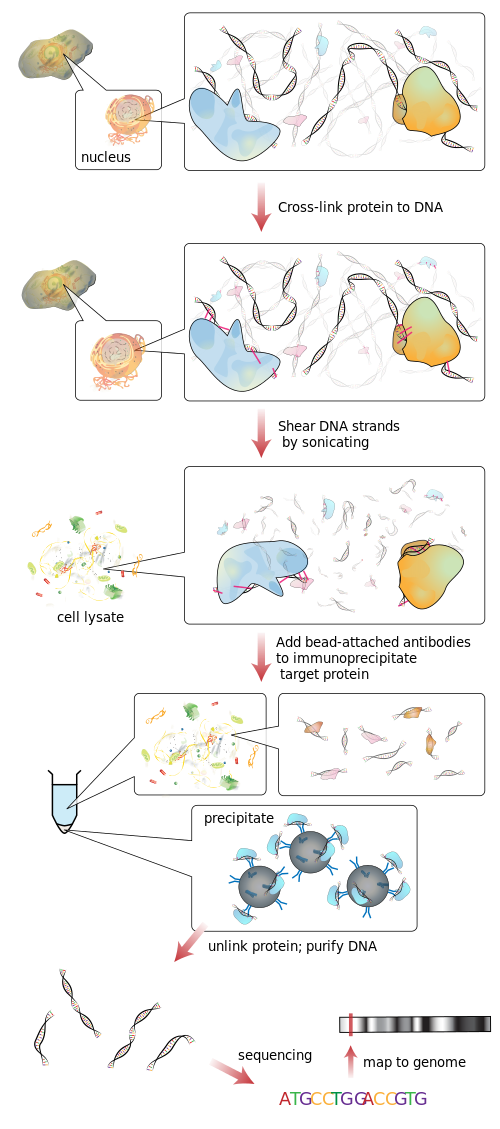
\includegraphics[scale=0.6]{image1}

\caption{Peak classification uses a DNA alignment to classify identified binding
sites (Odom, Dowell et al, 2007)}


\end{figure}


Some binding sites have too weak of a signal to confidently identify,
but evidence from the genomes of related strains may provide the additional
support needed to identify these. Using the normalized difference
score (NormDiff) described by Zheng et al (2010), we were able to
find substantial evidence for conserved binding sites that were not
identified by MACS, a commonly-used tool for identifying binding sites
from ChIP-seq data, by comparing the NormDiff scores from peaks identified
in one experiment with the same region from another experiment (the
syntenic region). We were able to identify some additional peaks found
in one strain as conserved with a statistical analysis of the NormDiff
values. We also present modifications to the normalized difference
score that use the data from multiple genomes concurrently.


\section{Background}


\subsection{Genetic analysis of transcription factor binding variation in yeast
(Zheng et al. 2010)}

In 2010, Zheng et al. analyzed transcription factor binding sites
in two strains of yeast, S96 and HS959, by using ChIP-seq for a transcription
factor called Ste12. They found transcription factor binding sites
using MACS software (section 2.2, appendix A). About 40\% of the binding
sites are found to vary across different yeast strains according to
their analysis (Figure 2).

\begin{figure}


\includegraphics[scale=0.5]{consensus4}

\caption{A Venn diagram showing the number of identified Ste12 binding sites
in S96 (left) and HS959 (right). Binding sites are identified as conserved
(blue intersecting region) if they target the same gene for different
yeast strains S96 and HS959 (Zheng et al. 2010).}
\end{figure}


In order to get a comprehensive picture of the changes associated
with transcription factor binding variations, Zheng et al. created
NormDiff to find the background subtracted and normalized ChIP-seq
binding signal (see Methods). They found variable binding regions
by analyzing the variation of the binding signal across different
experiments. 

Their analysis was very informative, but instead of analyzing the
variable binding sites, we wanted to find additional conserved binding
sites. In order to do this, we looked at the binding sites found by
MACS and looked at the distribution of the NormDiff scores to find
patterns of conserved binding sites.


\subsection{Model based analysis of ChIP-seq (Zhang et al. 2007)}

Peak finding is an important part of finding transcription factor
binding sites. Model-based analysis of ChIP-seq (MACS) is a popular
and open source software tool for peak finding in ChIP-seq data. We
performed a source code study of MACS (see Appendix A) in order to
understand it\textquoteright{}s functionality in detail. We discuss
some of the details here.

Internally, MACS uses a list of tuples corresponding to the position
and orientation of each ChIP-seq tag. The length of the ChIP-seq fragments
is unknown because only a small part of the 5\textquoteright{} ends
are sequenced. To compensate, MACS calculates a shift model to estimate
the length of the ChIP-seq fragments. MACS uses a \textquoteleft{}na�ve\textquoteright{}
peak to find pairs of peaks using the paired-end reads. Then the median
distance between each pair estimates the total ChIP-seq fragment size.
Then MACS extends the length of each read towards the 3\textquoteright{}
end to represent the true length of the ChIP-seq fragments.

For finding peaks, MACS uses a Poisson distribution model to find
data that is highly different from the background distribution. The
background is calculated as the expected number of reads in the scanning
window given the total number of reads and the whole genome size.
Then peaks are identified as the likelihood of receiving a large number
of reads in our scan window compared with the background. The result
is a list of high confidence ChIP-seq peaks that represent potential
transcription factor binding sites. 


\subsection{Finding conserved transcription factor binding sites}

Comparing data from multiple experiments to find conserved binding
sites is important for understanding evolution, measuring data similarity,
experimental reproducibility, and finding biological invariants. However,
ChIP-seq experiments are subject to many variables such as noise,
bias, and differences in sequencing depth (Shao et al. 2012). These
variables can make comparing different ChIP-seq experiments difficult,
so it is important to find a good model to account for these variables.

Methods for analyzing chromatin immunoprecipitation using microarray
(ChIP-chip) are well studied for using normalization, scaling, and
discretization (Zhou and Wong, 2008). Finding conserved binding sites
involves additional analysis however. The basic method that has been
used for finding conserved binding sites is to align the genomes and
find overlapping peaks for common target genes. One method for finding
conserved binding sites using the peak classification mentioned above
for ChIP-chip was introduced by Odom, Dowell et al. (Figure 1).

To assess the quality of the conserved binding site, we can also compare
the p-values and the empirical false discovery rate to assess the
binding site similarity. However, if we want to find conserved binding
sites that have a weak binding signal, then MACS might not be very
useful, because we would have to use a low significance threshold
for MACS, which can result in many false positives. Additionally,
using a low significance threshold for MACS results in very broad
peaks (see Appendix A, section 3). 

In our previous work (Statistics and Computation for Genomes and Metagenomes,
Spring 2012), we tried to use the correlation of data from the binding
sites and the syntenic region as a measure of a conserved binding
site. While this method was able to identify some conserved binding
sites, it was not consistent and exhibited too much noise to shown
a clear correlation.

\begin{figure}
\includegraphics[scale=0.35]{image3_2}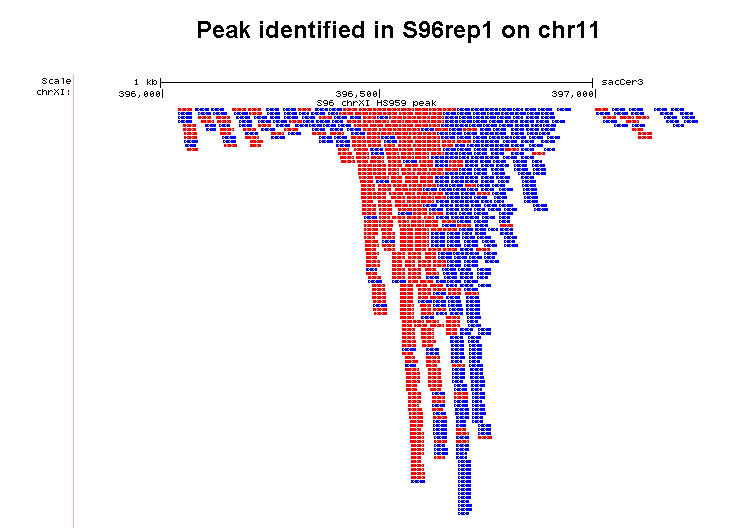
\includegraphics[scale=0.35]{image4_2}

\caption{(left) The correlation score from peaks in HS959 and S96 does not
show a strong positive correlation, with most correlations near zero.
(right) The shared peaks from replicate experiments have more of a
strong positive correlation, with many more peaks showing high positive
correlations.}


\end{figure}


A more recent technique used for finding conserved binding sites using
ChIP-seq is MANorm (Shao et al, 2012). MANorm uses binding sites identified
by a peak finding program and raw ChIP-seq data to fit a linear model
for shared peaks (Figure 3). MA plots use log-product and log-ratio
to compare two experiments, and these techniques have been historically
used for analyzing ChIP-chip arrays but MANorm adapted it to normalize
ChIP-seq data in MANorm. MANorm can also find conserved binding sites
in terms of a Bayesian Poisson model.

\begin{figure}


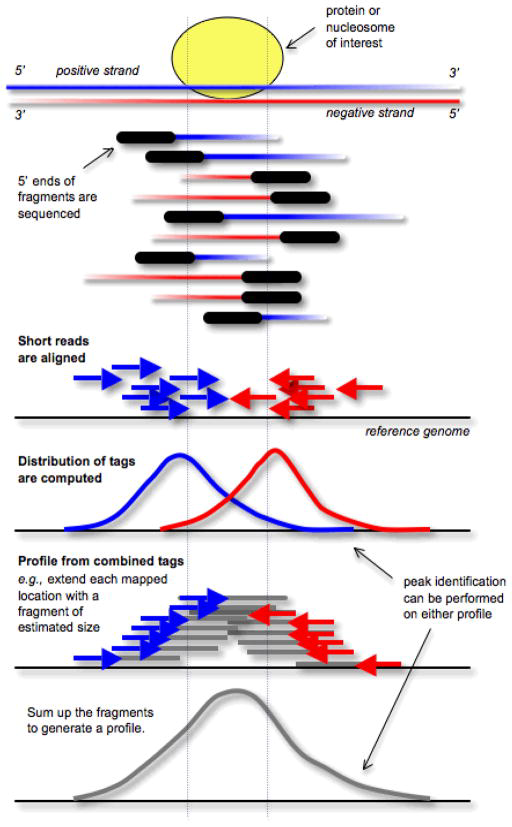
\includegraphics[scale=0.4]{image2}

\caption{MANorm uses the data and peak finding results from two experiments
to normalize the data and to find additional conserved binding sites.}


\end{figure}



\section{Accomplishments}


\subsection{Evidence for unidentified shared peaks}

To determine the scope or the problem of unidentified conserved binding
sites, we calculated the normalized difference score of Zheng et al.
using the number of ChIP-seq tags that overlap each genome position
(see Methods). Then we used a sliding window to calculate the maximum
average NormDiff score for the peaks that are found using MACS as
well as the syntenic region for comparison. We found in many cases
that syntenic regions are enriched with ChIP-seq reads even when it
is not called a binding site by MACS (Figure 4a). To look at both
experiments concurrently, we analyzed a MA plot of the NormDiff scores
that uses the log-product and log-ratio of the maximum average NormDiff
scores overlapping the peaks from both experiments (Figure 4b). The
MA plot shows many binding sites that are unique to one experiment
overlap the same region as the shared binding sites in the figure. 

\begin{figure}
\includegraphics[scale=0.35]{image6_2}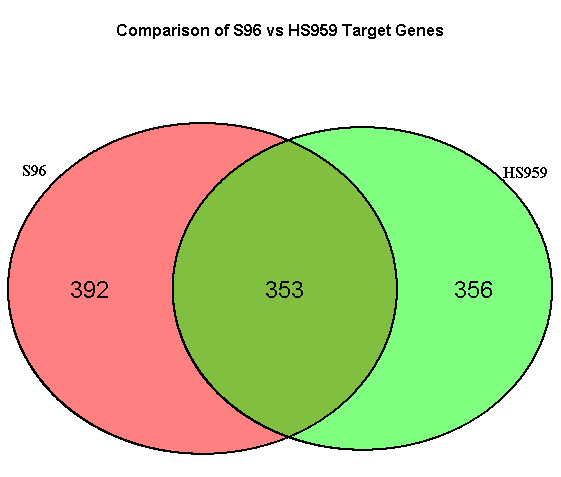
\includegraphics[scale=0.35]{image7_2}

\caption{Comparing the NormDiff score of peaks found using MACS with the syntenic
region of another experiment shows that even sites that aren\textquoteright{}t
called shared have significant NormDiff scores. Note how often there
are red or green points (representing binding sites called in only
one strain) overlapping the region of blue points (which represent
binding sites considered shared by MACS).}


\end{figure}


Peaks that were not identified by MACS but for which there might still
be a shared peak are in what is referred to as the \textquotedblleft{}twilight
zone\textquotedblright{} (Figure 5). Since NormDiff is normalized,
it allows for simple and direct comparison of data. The \textquotedblleft{}twilight
zone\textquotedblright{} represents the overlap of the NormDiff scores
from shared peaks that are at least as big as the syntenic region.
We sorted the the syntenic region\textquoteright{}s max average NormDiff
score for the shared and unique peaks separately (Figure 5). This
shows that some of the strongest NormDiff scores were not called shared
when other weaker signals were called. 

\begin{figure}
\includegraphics[scale=0.35]{image9_2}\includegraphics[scale=0.35]{image10_2}

\caption{The \textquotedblleft{}twilight zone\textquotedblright{} in yellow
shows the NormDiff scores of peaks found to be shared overlap with
NormDiff scores of peaks that were not identified}


\end{figure}


To compare the distribution of the peak NormDiff scores with the background,
we also looked at the distribution of NormDiff across the whole genome
(see Methods). This showed that the NormDiff scores that overlap peaks
were visibly different from the background (Figure 6). The syntenic
regions and the peak regions are also highly correlated even at low
levels of expression, which indicates that something that might not
be called a peak by a peak finder using strict cutoffs might still
be biologically significant. There are also a number of regions for
which the syntenic region in neither genome is called a peak that
overlap identified conserved binding sites, giving evidence that there
may be many conserved peaks that are not identified in either genome.

\begin{figure}
\includegraphics[scale=0.35]{image11_2}\includegraphics[scale=0.35]{image12_2}

\caption{Figure 6. The distribution of the NormDiff scores for the whole genome
are shown in contrast with the average NormDiff scores of the peak
and syntenic regions, showing that even peaks that are not called
shared are significantly elevated over the background, and more importantly,
that there may be many conserved binding sites that are not currently
identified in either genome (gray points that overlap the region with
red points).}


\end{figure}



\subsection{Using the normal distribution of NormDiff to identify additional
conserved peaks}

We developed a new model for assessing conserved binding sites by
using the normalized difference score from Zheng et al. Using the
observed normal distribution of NormDiff scores, we identified high
confidence binding sites as those that are statistically highly different
from the background (see Methods). We analyzed the regions syntenic
to peaks called in only one strain. We found 42 new binding sites
in HS959 with that were conserved in S96 that were not identified
by MACS with P<0.05, and 4 of these binding sites that were conserved
with P<0.01. We also found 76 binding sites in S96 with P<0.05 that
were conserved in HS959, and 13 of these binding sites were conserved
with P<0.01 

\begin{figure}
\includegraphics[scale=0.35]{image13_2}

\includegraphics[scale=0.35]{image14_2}

\caption{The maximum average NormDiff score calculated from the syntenic region
is used to identify additional binding sites that are conserved in
each experiment.}


\end{figure}


To evaluate the significance of these findings, we evaluated all binding
sites that were previously identified from S96 using our algorithm
and we found 98\% (885/897) at P<0.05, and 60\% (563/897) binding
sites at a P<0.01. In HS959 we identified 85\% (729/824) of the same
binding sites at P<0.05 and 46\% (365/824) at P<0.01. This indicates
that our algorithm is able to identify many significant binding sites
that are found by other peak finding algorithms.

We also compared our results with results about transcription factor
binding sites from previous studies (Harbison, Gorden et al.) and
we found many of our results overlap known yeast regulatory regions
(see Figure 8). This shows that the normalization of the data can
be used to identify shared binding sites that aren\textquoteright{}t
identified by other algorithms. 

\begin{figure}
\includegraphics[scale=0.35]{image15_2}

\caption{ChIP-seq peak identified by MACS (bottom) and the peak that was identified
by our algorithm that MACS did not identify (top). Bottom track shows
overlap with known regulatory regions. }


\end{figure}



\subsubsection{Drawbacks of this approach}

Our approach tries to find evidence for conserved binding sites by
analyzing data using normalized difference scores. Our approach gives
some evidence of peaks with high confidence P-values, which is shown
in our results of finding new peaks with P<0.01. However, these findings
have much less confidence than thresholds set by MACS (P<1e-5). 

One of the reasons that we have less confidence in P-values is because
NormDiff uses control data for background subtraction. MACS does not
use control data to calculate P-values, but it uses control data to
calculate false discovery rates. The background subtraction used in
NormDiff may result in higher P-values because of the loss of signal
from background subtraction. Additionally, we use a normal approximation
for our data, but since our data is not continuous it may not behave
as well as Poisson distribution. 


\subsection{Modified NormDiff scores to identify conserved binding sites simultaneously}

In addition to identifying conserved binding sites that were previously
identified in only one genome, we wish to also identify conserved
binding sites that are too weak to identify individually in either
genome, but for which the combined data from multiple genomes can
together provide sufficient evidence for the binding site. As a first
step towards this, we created modified NormDiff scores that use the
data from two genomes concurrently (see Methods). 

One modified NormDiff score calculates the added effect of two experiments
(Zadd), and with the other calculates the subtracted effect (Zsub).
Zadd provides information about the added effect of two experiments,
so if Zadd is high, then if considered together the binding sites
can be considered to be significant. Zsub provides information about
the similarity of the peaks: if the subtractive score is small, then
the binding sites have a small difference, and they are similar. We
hypothesize that comparing and/or combining these two scores can be
used to identify conserved and differential binding. (Figure 9). For
example, if the subtractive score is small but the additive score
is large, then the binding site is likely to be conserved in both
experiments. 

We can test our hypothesis that Zsub is small by using a hypothesis
test: we assume the mean is 0, and test whether the observed distribution
is different. We can also check that the sum of each random variable
is large (setting a significance threshold) according to a hypothesis
test also.

We analyzed S96 peaks and HS959 peaks using the modified NormDiff
score and found that the data clusters around zero on Zsub, indicating
a high degree of similarity. The peaks that are highly different from
each other appear far from zero on Zsub. The difference in the Zsub
score could indicate a significant difference in the binding site. 

\begin{figure}
\includegraphics[scale=0.35]{image16_2}\includegraphics[scale=0.35]{image17_2}

\caption{$Z_{add}$ vs. $Z_{sub}$ for S96 and HS959. The modified NormDiff
scores are used to find evidence of shared binding sites in the HS959
and S96 genomes. Both genomes are considered concurrently with the
modified NormDiff score to find shared peaks}
\end{figure}


If we wanted to do hypothesis testing on this plot, the Zsub scores
that cluster around 0 and the Zadd scores that are highly significant
according to our hypothesis tests might effectively show up as according
to the bands shown in Figure 10. We could also do multiple hypothesis
testing using Bonferroni correction or other techniques for analyzing
the significance of both tests at the same time.

\begin{figure}
\includegraphics[scale=0.35]{image18_2}\includegraphics[scale=0.35]{image19_2}

\caption{(left) Using hypothesis testing for Zsub would give a range of values
shown as black bars, and the hypothesis testing for Zadd would give
a significance level shown as a green bar. (right) Hypothetical range
of conserved peaks identified by multiple hypothesis testing}


\end{figure}



\section{Discussion}


\subsection{Additional possible modifications for NormDiff scores}

We also have considered other modifications to NormDiff to include
log scale, analogous to the information shown in an MA plot. We observed
that the NormDiff score is actually very similar to previous evaluations
for oligonucleotide arrays (Bolstad et al. 2003). The AvDiff score
commonly used for Affymetrix arrays which compares the perfect match
(PM) to mismatch (MM) to estimate the binding strength for each probe
set A using the following

AvDiff = 1/A Sigma(PM-MM, 1\ldots{}A)

AvDiff tells us the average level of expression of a probe, which
is similar to how NormDiff tells us the average strength of the ChIP-seq
binding signal at a genome position given the observed reads. Bolstad
et al. argue that the log scale improves analysis in a widespread
number of ways for oligonucleotide data, including normalization,
bias, and model fit. They proposed using

AvLog=1/A Sigma(log(PM-MM), 1\ldots{}A)

Using a log-scale for NormDiff could possibly improve its performance,
however, some issues with log-scale exist. For example, the log-scale
exaggerates small differences and decreases larger differences. ChIP-seq
is purported to have a higher dynamic range (Park et al. 2009) but
using a log-scale transformation significantly alters dynamic range,
which could decrease our ability to identify conserved and differential
binding sites 

\begin{figure}
\includegraphics[scale=0.35]{image20_2}

\caption{Peaks shown in green show highly differential Zsub scores that are
identified as shared. Scrutinizing these binding sites for differences
could show that they are not conserved.}


\end{figure}



\subsection{Conserved sequences}

In our analysis, we do not consider the effect of the conserved sequences
or the motif patterns of the binding sites. However the different
genomes of yeast that we analyzed have diverged sequences so sequence
comparisons would be informative. Additionally, for finding weakly
conserved binding sites, assessing the degree of sequence conservation
can indicate the biological importance of certain functions, because
transcription factor binding sites have much higher conservation rates. 

Recent studies on human cell lines show regulatory footprints of transcription
factor binding sites have much higher conservation rates (Neph et
al. 2012). This study also found transcription factors that are indirectly
bound to the DNA by finding ChIP-seq peaks that have with no regulatory
footprint or motif underlying the ChIP-seq peaks (Neph et al. 2012).
These results show how integrating data about sequence conservation
can show additional info about the binding sites that are not found
in only ChIP-seq data.


\section{Conclusion}

Finding conserved transcription factor binding sites is important
for comparing ChIP-seq data for transcription factors that influence
gene regulation. Some binding sites that are identified as not being
shared have too weak of a signal to identify confidently, but by comparing
multiple experiments there we can see that they are significant. 

We found substantial evidence for shared binding sites that were not
called by other peak finding algorithms using the normalized difference
score, a method for finding conserved binding sites from multiple
ChIP-seq experiments. We then applied a statistical analysis to the
distribution of normalized difference scores to confidently identify
additional conserved binding sites that were identified by MACS in
one genome but not the other. However, while significant, the confidence
levels that we obtained using Normal peak calls were not as significant
as we\textquoteright{}d hoped. We developed modifications to NormDiff
that may provide evidence for shared binding sites that are not called
by other algorithms. 


\section{Methods}


\subsection{Matching positions in different ChIP-seq experiments}

In ChIP-seq data many datapoints may be missing when no sequence aligns
to them. Instead of filling in missing data as zero or N/A we used
algorithm for \textquoteleft{}matching\textquoteright{} positions
from different ChIP-seq experiments. The interval search, which matches
a vector X to a vector Y, is efficient for matching sorted data vectors.
It uses the expression apply(outer\_product(x,y,>=),sum).

Then if we calculate interval search(\{5\}, \{1,2,3,5,6\}) then we
take the outer product of X,Y to make all combinations of expressions
5>=1, 5>=2, 5>=3, 5>=5 , 5>=6 

Each expression is TRUE(1) or FALSE(0), and the sum gives the position
of X in Y sum(TRUE, TRUE,TRUE, TRUE, FALSE)= 4 

Performing interval search(\{4,5,6\},\{1,3,5,6\}) would result in
a 3x4 list, however the algorithm is implemented as a binary search
that uses each TRUE or FALSE value as branches. This algorithm has
effective running time as O(n log N) for n=len(x) and N=len(y)


\subsection{Normalized difference scores}

The normalized difference (NormDiff) score is a useful statistic for
comparing ChIP-seq data that uses background subtraction and normalization
to obtain the ChIP-seq binding signal. The NormDiff score from Zheng
et al. uses a simple random model for ChIP-seq ($A$) and control
($B$) defined as

\begin{eqnarray*}
A & \sim & Poisson(f+g)\\
B & \sim & Poisson(cg)
\end{eqnarray*}


Where- 

$f$ represents the binding signal

$g$ represents the background noise

$c$ is a scaling factor between $A$ and $B$\\


Then, the NormDiff $Z$ is defined for each genome position $x_{i}$
as 

\[
Z(x_{i})=\frac{A(x_{i})-B(x_{i})/c}{\sigma}
\]
 

Then the scaling factor $c$ is estimated as the median ratio of $A/B$
and the variance $\sigma$ is estimated from $\sqrt{A+B/c^{2}}$.


\subsection{Sliding windows for NormDiff}

For analyzing the strength of the ChIP-seq binding signal using NormDiff,
we averaged the NormDiff score over sliding 100bp windows that are
within or overlap each peak and syntenic region and used the maximum
value that it obtains for comparison. Because NormDiff requires both
control and treat data, we used the only positions that matched, or
in the case of a missing data, the nearest matching position is used
according to the interval search (section 6.1). 

To analyze the whole genome as in Figure 6, we go through each chromosome
from start to end and analyze non-overlapping 100bp windows. Then
separately, we find the maximum average normdiff score overlapping
the peak regions and color these according to whether or not the window
overlaps a peak in one or both genomes.


\subsection{Statistical analysis of NormDiff}

The distribution of NormDiff scores uses a signal plus background
(f+g) approximation with background subtraction. NormDiff is approximately
normally distributed for the null hypothesis, where f=0, however the
binding signal f causes significant deviations from the normal (Figure
12). We can also see that the sampling distribution of NormDiff scores
is approximately normal with significantly less variance (Figure 13).
We use the maximum average NormDiff score overlapping peaks and compare
that with the normal distribution to detect peaks as P(Z>= \={x}) 

\begin{figure}
\includegraphics[scale=0.35]{image24_2}\includegraphics[scale=0.35]{image26_2}

\caption{(left) The distribution of NormDiff scores for the entire genome shows
approximately normal distribution. (right) Q-Q Plot shows that the
binding signal deviates significantly from the expected normal distribution.}


\end{figure}



\subsection{Modified normalized difference score}

We considered a modified NormDiff score that combines data from multiple
experiments concurrently to find conserved binding sites. For example,
a NormDiff score that adds data from two experiments, with binding
data A1 and A2, respectively, and with background (control) data B1
and B2, respectively, can be defined as \\
\[
Z_{add}(x_{i})=\frac{(A_{1}-B_{1}/c_{1})+(A_{2}-B_{2}/c_{2})}{\sigma}
\]


Then the scaling factors $c_{1}$and $c_{2}$ are estimated from data,
and the variance is $\sigma=\sqrt{A_{1}+B_{1}/c_{1}^{2}+A_{2}+B_{2}/c{}_{2}^{2}}$ 

A NormDiff score that subtracts data from two experiments could also
be defined as
\[
Z_{sub}(x_{i})=\frac{(A_{1}-B_{1}/c_{1})-(A_{2}-B_{2}/c_{2})}{\sigma}
\]


Note: The variance for $Z_{sub}$ would be the same as the variance
for $Z_{add}$. 


\section{Bibliography}

\bibliographystyle{plain}
\nocite{*}
\bibliography{References}


\appendix

\section{Source code study of MACS}

We did a source-code study of MACS (Model-based analysis of ChIP-seq)
for version 1.4.2 to find out details about its implementation and
processing. The published description of the program is thorough,
but we found additional info in the code that helped us understand
the details of ChIP-seq processing. 


\subsection{Loading ChIP-seq data}

To begin MACS loads ChIP-seq tags from experiment and control files
specified by the \textendash{}t and \textendash{}c options (macs14.py,
load\_tag\_files\_options). This builds an internal representation
of the tags in a key-value store known as a dictionary. The table
is a list of tuples of the position and orientation of each tag with
the chromosome that it is in. It then calculates max duplicate tags
for each position (macs14.py, cal\_max\_dup\_tags) and filters duplicate
tags according to previous step (FeatIO.py, filter\_dup)

\begin{figure}
\includegraphics[scale=0.4]{image33_2}

\caption{The call graph for loading ChIP-seq data for a typical run. Percentages
are given as a percent of whole program runtime. The main functions
include parsing and sorting the tags by position.}


\end{figure}



\subsection{Build shift model}

MACS calculates a \textquotedblleft{}shift model\textquotedblright{}
to estimate the ChIP-seq fragment size from paired-end reads using
the PeakModel class. PeakModel uses a method \_\_naive\_find\_peaks
peak finder to scan for peaks on each strand that are at least \textendash{}mfold
(default value 10) greater than the background. The background is
calculated according to other inputted parameters \textendash{}g and
\textendash{}bw representing the genome size (1.2e7 for yeast) and
bandwidth (default 300).

\begin{lstlisting}
background_reads = total_reads*bandwidth/genome_size 
min_tags = mfold*background_reads  
\end{lstlisting}


Then PeakModel processes all on the same strand that are within the
window size (2{*}bandwidth) and adds them to a 'line'. It finds pairs
of peaks for all 'lines' greater than min\_tags that are within 4{*}bandwidth
and then the shiftsize 'd' is calculated as the median length between
them.

\begin{figure}
\includegraphics[scale=0.4]{image34_2}

\caption{The PeakModel subgraph. It shows how the paired peaks are identified
using a na�ve peak finder (right branch), and then modeled as \textquotedblleft{}lines\textquotedblright{}
to estimate the distance between them (left branch). }
\end{figure}



\subsection{Find peaks according to Poisson distribution}

To do peak finding, MACS uses candidate peak finder with a basic Poisson
distribution model with a rate parameter calculated as the expected
number of background reads bg0 calculated as follows where scan\_window
is equal to 'd' and p-value is an inputted threshold from \textendash{}p
(default value is 1e-5)

\begin{lstlisting}
lambda_bg0=scan_window*total_reads_treatment/genome_size 
min_tags = poisson_cdf_inv(1-pow(10,self.pvalue/-10),lambda_bg0)+1 
\end{lstlisting}


All the candidate peaks that exceed min\_tags are merged if they overlap.
It has been noted that merging all overlapping peaks leads to excessively
broad peaks under normal conditions if too low of a significance threshold
is used. Next, the filtering step looks candidate peaks to make sure
they are significantly enriched versus the control data. 

For filtering the candidate peaks, the Poisson rate is calculated
using t\_ratio \textendash{} the scaling factor of total reads between
the control and treatment data. We build a Poisson model using the
number of reads we would expect using the length of the candidate
peak given the total background and local regions around the candidate
peak. 

\begin{algorithm}
\begin{lstlisting}
PeakDetect.__filter_w_control(peak_candidates, treat, control, ratiotreat2control)

t_ratio=total_reads_control/total_reads_treatment  
lambda_bg = lambda_bg0/d*candidate_peak_width*t_ratio

For each candidate peak {
      //Calculate #reads in the candidate peak window
      //Calculate #reads in small, large region (5000,10000kb window)
      clambda_peak = total_tags_control_in_peak
      tlambda_peak = total_tags_treatment_in_peak*t_ratio
      ...
} 
\end{lstlisting}


\caption{Code listing - pseudocode summary of peak caller}


\end{algorithm}


Interestingly, the peak finder uses the scaled number of tags calculated
using t\_ratio instead of the total number of tags. Then the local
lambda (described in MACS paper as being robust against local biases,
possibly referring to chromatin bias, etc) is calculated as the max
of the lambdas of the peaks found in the control data.

\begin{lstlisting}
Local_lambda=max(lambda_bg,clambda_peak,clambda_lregion,clambda_sregion)
\end{lstlisting}


Then to calculate final\_peaks, MACS calculates the Poisson cumulative
distribution function for the number of reads in the window for the
local\_lambda, which returns a probability that this is a peak. If
the probability is greater than user defined p-value, then it is a
final\_peak (returned to user)

\begin{lstlisting}
p_tmp = poisson_cdf(tlambda_peak,local_lambda,lower=False)
peak_pvalue = mathlog(p_tmp,10) * -10
if(peak_pvalue > self.pvalue)
     final_peaks.append candidate_peak 
\end{lstlisting}


Finally, MACS calculates an empirical false discovery rate for each
peak. This is calculated using a sample swap: it uses ChIP-seq data
as control and control data as ChIP-seq and identifies the \emph{number
of peaks in the control} / \emph{number of peaks in chip-seq} for
each p-value that is calculated for each peak. The empirical FDR is
important since it lets us see for each peak the number of peaks that
would be called at each significance threshold.

\begin{figure}
\includegraphics[scale=0.4]{image36_2}

\caption{The call graph for the PeakDetect subgraph shows the time spent on
peak calling. Note that call peaks w control is performed twice: once
for peak calling, and once for estimating the empirical false discovery
rate.}


\end{figure}

\end{document}
